\documentclass[final,t]{beamer}
\mode<presentation>{\usetheme{Purdue}}

\usepackage{natbib,url}
\usepackage{multicol}
\usepackage{geometry}
\usepackage{multirow}
\usepackage{rotating}
\usepackage{wrapfig}

\usepackage{tikz}
\usetikzlibrary{shapes,arrows}
\usepackage{graphicx}
\usepackage{tikz-dependency}
\usepackage{natbib}
\usepackage{url}
%\usepackage{gb4e}
\usepackage{amsmath}
\DeclareMathOperator*{\argmax}{arg\,max}
\DeclareMathOperator*{\argmin}{arg\,min}
% MD: This threw an odd error for me:
%\usepackage{tikz-qtree}
\usepackage[framemethod=tikz]{mdframed}

\newcommand{\myboxedtext}[2][rectangle,draw,rounded corners]{%
            \tikz[baseline=-0.6ex] \node [#1,rounded corners]{#2};}%

\usepackage{enumerate}
\usepackage{color}
\usepackage{xcolor}
\usepackage{caption}

\definecolor{light-gray}{gray}{0.9}
\definecolor{forestgreen}{rgb}{0.13, 0.55, 0.13}
\definecolor{carnelian}{rgb}{0.7, 0.11, 0.11}
\definecolor{darkblue}{rgb}{0.0, 0.0, 0.55}
\definecolor{darkgreen}{rgb}{0.0, 0.2, 0.13}
\definecolor{persimmon}{rgb}{0.93, 0.35, 0.0}

\usepackage[size=custom,width=120,height=90,scale=1]{beamerposter}
\usepackage{gb4e}

\title[]{Annotating Picture Description Task Responses for Content Analysis}
\author[]{Levi King \& Markus Dickinson}
\institute[]{Indiana University}
\date[]{5 June 2018}
\newcommand{\myimg}{
  \framebox{
   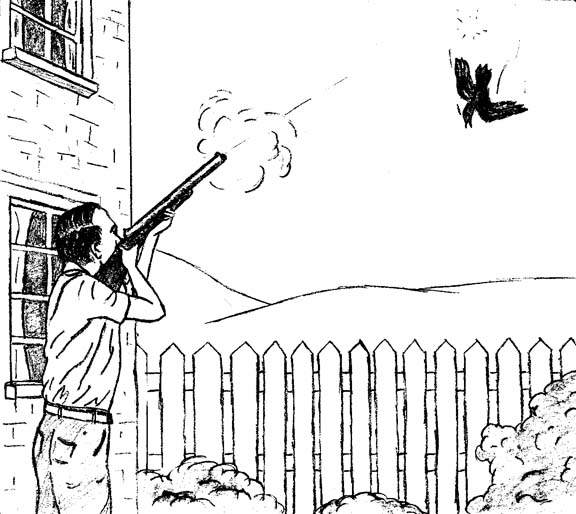
\includegraphics[width=.95\textwidth]{../figures/exampleprompt2.jpg}}}
\setbeamertemplate{caption}[numbered]
\setbeamertemplate{itemize/enumerate body begin}{\normalsize}
\setbeamertemplate{itemize/enumerate subbody begin}{\normalsize}
\setbeamertemplate{itemize/enumerate subsubbody begin}{\normalsize}

%%%LK: May 2, 2018: I've changed the block names, but the content is still all from 2016. 

\begin{document}
\begin{frame}{}
\vspace{-1.3em}
  \begin{columns}[t]
    \begin{column}{.33\linewidth}

\begin{block}{Overview \& Background}
  \begin{itemize}
    \itemsep1em
  \item{\textbf{Goal:} Evaluate semantic accuracy of non-native speaker (NNS) responses to picture description task (PDT) 
      \begin{itemize}
      \item Compare to gold standard (GS) of native speaker (NS) responses
      \end{itemize}
    }
\end{itemize}
    \begin{center}
      \mbox{}\\[-1em]\textbf{Past Approach}
    \end{center}
      \begin{center}\begin{minipage}{.8\textwidth}
      \begin{enumerate}
      \item Dependency parse NNS responses \& GS
      \item Use custom rules to extract and lemmatize
        \textit{verb-subject-object} triple for each response
      \item Attempt to match NNS triple to GS triples
      \end{enumerate}
      \end{minipage}\end{center}

    \begin{center}
      \textbf{Past Limitations} 
    \end{center}
      \begin{center}\begin{minipage}{.8\textwidth}
      \begin{enumerate}
      \item GS is small
      \item NNS responses show more variation than NS responses
      \item Matching exact triples is restrictive (no partial matching)
        \begin{itemize}
        \item{\textit{kick(boy, ball) $\neq$ kick(boy, football)}}
        \end{itemize}
      \end{enumerate}
      \begin{center}
        Upshot: low coverage (50.8\%)
      \end{center}
      \end{minipage}\end{center}

  \begin{center}
    \mbox{}\\\textbf{Current Approach} 
  \end{center}
    Generalize methods by:\\[0.5em]
    \begin{minipage}{.9\textwidth}
    \begin{enumerate}
    \item Representing responses as lists of dependencies
    \item Scoring NNS response representation according to how closely it resembles GS representation
  	\begin{itemize}
		\item{partial matching: \textbf{\textcolor{forestgreen}{subj\_boy\_kick} \texttt{+} \textcolor{carnelian}{obj\_ball\_kick}} vs. \textbf{\textcolor{forestgreen}{subj\_boy\_kick} \texttt{+} \textcolor{carnelian}{obj\_football\_kick}}}

	\end{itemize}
    \end{enumerate}
  \end{minipage}
\end{block}

\begin{block}{Picture Description Task}
\begin{center}
  \textcolor{purple}{Picture Description Task (PDT)}
\end{center}
	\vspace{-.38em}
    \begin{itemize}
    \item{10 items (2 photos, 8 drawings) depicting transitive events}
    \item{PDT elicits natural productions but constrains form \& content}
    \end{itemize}
\begin{center}
  \textcolor{purple}{Participants}
\end{center}
	\vspace{-.38em}
    \begin{itemize}
    \item{39 NNSs, intermediate/advanced English; 390 sentences}
      \begin{itemize}
      \item{Arabic, Chinese, Japanese, Korean, Spanish, Kurdish, Polish, Portugese}
      \end{itemize}
      \smallskip
    \item{14 NSs; 140 sentences}
    \end{itemize}
	\bigskip
\setlength{\fboxsep}{3pt}
\setlength{\fboxrule}{0pt}
	
	\begin{table}
	\begin{tabular}{|@{}c@{}|}
		\hline
		\myimg \\ %%%LK: this is defined before '\begin{document}'
		\hline
		\textbf{Example Response (L1)} \\
		\hline
		The man killing the beard. (Arabic)\\
		\hline
		A man is shutting a bird. (Chinese) \\
		\hline
		A man is shooting a bird. (English) \\
		\hline
		The man shouted the bird. (Spanish)\\
		\hline
	\end{tabular}
	\end{table}
	\vspace{-1em}
\end{block}

\end{column}

\begin{column}{.64\linewidth}
\begin{columns}
\begin{column}{.48\linewidth}

\vspace{-1em}
\begin{block}{Participants}
In the sections below, we explain the system parameter settings. The first two are closely related to generalizing the methods to overcome a limited GS, handle a wider range of sentence types (beyond transitives), and better reflect similarity to the GS.
\begin{center}
\begin{minipage}{.8\textwidth}
\begin{itemize}
	\item{Response Representation: By moving to a ``bag of dependencies'' approach, we loosen the strict evaluation from \textit{covered/not covered}; partial dependencies further loosen matching.}
	\item{Response Scoring: Averaging response term scores or calculating cosine distances allows for gradable rather than binary response scoring.}
\end{itemize}
\end{minipage}
\end{center}
\vspace{-.5em}
\end{block}

\begin{block}{Responses}
Responses are dependency parsed and treated as a list of \textit{terms}, which are dependencies in one of the formats below (\textit{l, d, h = label, dependent, head; x = placeholder}):
% MD: this is pretty hacky, but you need the double usage of center & minipage, as: 1) the first usage sets the size for what mdframed is going to box in, and 2) the second usage sets the location within the box
\begin{center}

\begin{minipage}{.33\textwidth}
% MD: To adjust spacing between top/bottom of box & the content, adjust the margins here:
  \begin{mdframed}[innertopmargin=15pt,innerbottommargin=15pt,roundcorner=10pt]
  \begin{center}
% MD: To adjust where the bullets show up, adjust this textwidth:
  \begin{minipage}{.8\textwidth}
    \begin{itemize}
    \item{\textbf{ldh:} \texttt{subj\_boy\_kick}}
    \item{\textbf{xdh:} \texttt{x\_boy\_kick}}
    \item{\textbf{lxh:} \texttt{subj\_x\_kick}}
    \item{\textbf{ldx:} \texttt{subj\_boy\_x}}
    \item{\textbf{xdx:} \texttt{x\_boy\_x}}
    \end{itemize}
  \end{minipage}
  \end{center}
  \end{mdframed}
\end{minipage}
\end{center}

\vspace{-.5em}
\end{block} 

\begin{block}{Annotation}

Scoring responses involves: 
\begin{center}
  \begin{minipage}{.85\textwidth}
    \begin{itemize}
    \item Weighting terms (dependencies) 
    \item Scoring responses: comparing weighted NNS terms with
      weighted GS terms
    \end{itemize}
  \end{minipage}
\end{center}

\begin{center}
\begin{minipage}{.78\textwidth}
  \begin{mdframed}[innertopmargin=15pt,innerbottommargin=15pt,roundcorner=10pt]
  \begin{center}
  \begin{minipage}{.9\textwidth}
    \begin{itemize}
    \item \textbf{Frequency Average (FA):} 
        \begin{itemize}
        \item Weight: NNS terms assigned GS term frequencies
        \item Response score: average of NNS term scores
        \end{itemize}
      \item \textbf{Tf-idf Average (TA):} 
        \begin{itemize}
        \item Weight: NNS terms assigned tf-idf scores based on GS
          frequencies
        \item Response score: average of NNS term scores
        \end{itemize}
      \item \textbf{Frequency Cosine (FC):} 
        \begin{itemize}
        \item Weight: NNS \& GS term frequencies are calculated
        \item Response score: cosine distance between NNS \& GS term
          scores
        \end{itemize}
      \item \textbf{Tf-idf Cosine (TC):} 
        \begin{itemize}
        \item Weighting: NNS \& GS tf-idf values are calculated
        \item Response score: cosine distance between NNS \& GS term
          scores
        \end{itemize}
    \end{itemize}
  \end{minipage}
  \end{center}
  \end{mdframed}
\end{minipage}
\end{center}
\vspace{-.5em}
\end{block}

\begin{block}{Agreement}
\texttt{TA} and \texttt{TC} require a reference corpus for deriving tf-idf scores. We experimented with two:
\begin{center}
\begin{minipage}{.49\textwidth}
  \begin{mdframed}[innertopmargin=15pt,innerbottommargin=15pt,roundcorner=10pt]
  \begin{center}
  \begin{minipage}{.8\textwidth}
    \begin{itemize}
    \item{\textbf{Brown Corpus (B)}}
    \item{\textbf{Wall Street Journal Corpus (W)}}
    \end{itemize}
  \end{minipage}
  \end{center}
  \end{mdframed}
\end{minipage}
\end{center}
\vspace{-.5em}
\end{block}

\begin{block}{Future Directions}
We experiment with two forms of the NNS responses:
\begin{center}
\begin{minipage}{.6\textwidth}
  \begin{mdframed}[innertopmargin=15pt,innerbottommargin=15pt,roundcorner=10pt]
  \begin{center}
  \begin{minipage}{.85\textwidth}
    \begin{itemize}
	\item{\textbf{NNSO:} Original, uncorrected form}
	\item{\textbf{NNSLM:} Language Model autocorrected form}
    \end{itemize}
  \end{minipage}
  \end{center}
  \end{mdframed}
\end{minipage}
\end{center}
\vspace{-.5em}
\end{block}

\end{column}

\begin{column}{.49\linewidth}
\vspace{-1em}
\begin{block}{PLACEHOLDER}
\begin{center}
\begin{minipage}{.9\textwidth}
\begin{enumerate}
	\item{Manually annotate responses; unacceptable responses are ``errors''}
	\item{Use each combination of parameters to produce a scored, ranked list of responses (Table \ref{tab:i10responses-avgprec})}
	\begin{itemize}
		\item{Good parameter settings should rank good responses near GS and errors far from GS}
	\end{itemize}
	\item{Evaluate and rank parameter settings by (mean) average precision ((M)AP) (Table \ref{tab:all-dist-ranked-settings})}
	\begin{itemize}
		\item{Also evaluate settings by non-normalized error score, which better illustrates differences in difficulty of PDT items (used in Figure \ref{fig:parameter-clusters})}
	\end{itemize}
	\item{Evaluate individual parameter values by MAP (Table \ref{tab:dist-ranked-parameters})}
\end{enumerate}
\end{minipage}
\end{center}
\vspace{.8em}

\begin{table}[htb!]
\begin{center}
\setlength{\tabcolsep}{0.3em}
\begin{tabular}{|r|c|l|r|r|}
 \hline
 \textit{R} & \textit{S} & Sentence & \textit{E} & \textit{V}\\
 \hline
 \hline
\multirow{2}{*}{1} & 1.000 & she is hurting. & 1 & 1.5 \\
& 1.000 & man mull bird & 1 & 1.5 \\
\hline
3 & 0.996 & the man is hurting duck. & 1 & 3.0 \\
4 & 0.990 & he is hurting the bird. & 1 & 3.0 \\
\hline
11 & 0.865 & the man is trying to hurt a bird & 1 & 11.0 \\
12 & 0.856 & a man hunted a bird. & 0 & 0.0 \\
\hline
17 & 0.775 & the bird not shot dead.  & 1 & 17.0 \\
18 & 0.706 & he shot at the bird & 0 & 0.0 \\
19 & 0.669 & a bird is shot by a un & 1 & 19.0 \\
20 & 0.646 & the old man shooting the birds & 0 & 0.0 \\
\hline
37 & 0.086 & the old man shot a bird. & 0 & 0.0 \\
38 & 0.084 & a old man shot a bird. & 0 & 0.0 \\
39 & 0.058 & a man shot a bird & 0 & 0.0 \\
  \hline
  \hline
  \multicolumn{3}{|c|}{Total Raw Score (not normalized)} & 17 & 169 \\
  \hline
  \multicolumn{3}{|c|}{Average Precision} & \multicolumn{2}{c|}{0.75084} \\
 \hline
\end{tabular}
\begin{minipage}{.9\textwidth}
\vspace{.7em}
\caption{Excerpt of rankings for Item 10 from the best system setting (TC\_B\_NNSLM\_ldh) based on average precision scores. \textit{R}: rank; \textit{S}: sentence score; \textit{E}: error; \textit{V}: rank value. }
\label{tab:i10responses-avgprec}
\end{minipage}
\end{center}
\end{table}
\end{block}

\begin{block}{PLACEHOLDER}
\vspace{.2em}
\begin{table}
\begin{center}
\begin{tabular}{|l|r||l|r||l|r||l|r|}
 \hline
 \multicolumn{2}{|c||}{Approach} & \multicolumn{2}{|c||}{Term Form} & \multicolumn{2}{|c||}{Ref. Corp. (TA/TC)} & \multicolumn{2}{|c|}{NNS Source} \\
 \hline
 \hline
 0.51577 & TC & xdh & 0.51810 & Brown & 0.51534 & NNSLM & 0.51937 \\
 \hline
 0.50780 & FC & ldh & 0.51677 & WSJ & 0.50798 & NNSO & 0.49699 \\
 \hline
 0.50755 & TA & lxh & 0.51350 & & & & \\
 \hline
 0.49464 & FA & xdx & 0.49901 & & & & \\
 \hline
 & 	& ldx & 0.49352 &  &  &  & \\
 \hline
\end{tabular}
\vspace{.7em}
\caption{Approaches and parameters ranked by mean average precision for all 10 PDT items.}
\label{tab:dist-ranked-parameters}
\end{center}
\end{table}

\vspace{.6em}
\begin{multicols}{2}
\begin{itemize}
	\item{Best approach: \textbf{TC}}
	\begin{itemize}
		\item{\textbf{TC} $>$ \textbf{FC}, \textbf{TA} $>$ \textbf{FA}:} 
		\begin{itemize}
			\item{tf-idf weighting $>$ frequency weighting}
		\end{itemize}
		\item{\textbf{TC}\&\textbf{FC} $>$ \textbf{TA}\&\textbf{FA}:}
		\begin{itemize}
			\item{cosine distance $>$ weight averaging}
		\end{itemize}
	\end{itemize}
	\item{Term form: \textbf{xdh, ldh, lxh} $>$ \textbf{xdx, ldx}}
	\begin{itemize}
        \item{Importance of heads (\textbf{h}): with short transitive
            responses, verbs are salient (subj/obj head)}
	\end{itemize}
	\item{Reference corpus: \textbf{Brown} $>$ \textbf{WSJ}}
	\begin{itemize}
        \item{Content \& style of responses more like \textbf{Brown}}
%            than \textbf{WSJ}}
	\end{itemize}
	\item{NNS source: \textbf{NNSLM} $>$ \textbf{NNSO}}
	\begin{itemize}
        \item{More errors in NNSLM forms, inflating MAP values:
            use non-normalized scores? (see paper)}
	\end{itemize}
\end{itemize}

\begin{table}[htb!]
\begin{center}
\begin{tabular}{|r|l|c|}
 \hline
 Rank & MAP & Settings \\
 \hline
 \hline
1 & 0.5534 & TC\_B\_NNSLM\_lxh \\
\hline
2 & 0.5445 & TA\_B\_NNSLM\_lxh \\
\hline
3 & 0.5435 & TC\_W\_NNSLM\_lxh \\
\hline
4 & 0.5422 & TC\_B\_NNSLM\_xdh \\
\hline
5 & 0.5368 & TC\_B\_NNSLM\_ldh \\
 \hline
 \hline
56 & 0.4816 & TA\_B\_NNSO\_xdx \\
\hline
57 & 0.4796 & FA\_na\_NNSLM\_ldx \\
\hline
58 & 0.4769 & FC\_na\_NNSO\_lxh \\
\hline
59 & 0.4721 & TA\_W\_NNSO\_xdx \\
\hline
60 & 0.4530 & FA\_na\_NNSO\_lxh \\
\hline
\end{tabular}
\begin{minipage}{.86\columnwidth}
\vspace{.7em}
\caption{Based on Mean Average Precision, the five best and five worst settings across all 10 PDT items.}
\label{tab:all-dist-ranked-settings}
\end{minipage}
\end{center}
\end{table}

\end{multicols}

\end{block}

\end{column}
\end{columns}

\begin{block}{PLACEHOLDER}
We used hierarchical clustering to explore for patterns among the items and parameters.\\
\mbox{}\hfill Set-up: cluster PDT items using features from response (e.g., type/token counts for terms) \& features from system performance (i.e., average error score for parameter setting).\hfill\mbox{}
\\\mbox{}\hfill Goal: new PDT items could be placed into known clusters via response features \& optimal parameter settings for that cluster could be applied automatically\\ 

\bigskip
\bigskip

\begin{minipage}{.45\textwidth}
\begin{figure}
\begin{center}
\begin{tikzpicture}[sloped]
\node (5) at (-16,0) {\textcolor{darkblue}{5}};
\node (9) at (-14.5,0) {\textcolor{darkblue}{9}};
\node (1) at (-12.5,0) {\textcolor{persimmon}{1}};
\node (4) at (-11,0) {\textcolor{persimmon}{4}};
\node (6) at (-9.0,0) {6};
\node (2) at (-7,0) {2};
\node (8) at (-5.5,0) {8};
\node (10) at (-3.5,0) {10};
\node (3) at (-1.5,0) {3};
\node (7) at (0,0) {7};
\node (59) at (-15.3,1) {};
\node (14) at (-11.8,1) {};
\node (28) at (-6.2,1) {};
\node (37) at (-0.8,1) {};
\node (1037) at (-2.3,1.7) {};
\node (281037) at (-4.5,2.5) {};
\node (6281037) at (-7.5,3.2) {};
\node (146281037) at (-10,4) {};
\node (59146281037) at (-13.5,4.7) {};
\draw  (5)  |- (59.center);
\draw  (9)  |- (59.center);
\draw  (1)  |- (14.center);
\draw  (4)  |- (14.center);
\draw  (2)  |- (28.center);
\draw  (8)  |- (28.center);
\draw  (3)  |- (37.center);
\draw  (7)  |- (37.center);
\draw (10) |- (1037.center);
\draw (37) |- (1037.center);
\draw (1037) |- (281037.center);
\draw (28) |- (281037.center);
\draw (6) |- (6281037.center);
\draw (281037) |- (6281037.center);
\draw (14) |- (146281037.center);
\draw (6281037) |- (146281037.center);
\draw (59) |- (59146281037.center);
\draw (146281037) |- (59146281037.center);
\end{tikzpicture}
\end{center}
\caption{PDT items clustered by type and token counts of all NS, NNSO and NNSLM responses.} 
\label{fig:response-clusters}
\end{figure}
\end{minipage}
\begin{minipage}{.45\textwidth}
\begin{figure}
\begin{center}
\begin{tikzpicture}[sloped]
\node (5) at (-16,0) {\textcolor{darkblue}{5}};
\node (9) at (-14.5,0) {\textcolor{darkblue}{9}};
\node (8) at (-12.5,0) {8};
\node (3) at (-10.5,0) {3};
\node (2) at (-8.5,0) {2};
\node (10) at (-7.0,0) {10};
\node (1) at (-5,0) {\textcolor{persimmon}{1}};
\node (4) at (-3.5,0) {\textcolor{persimmon}{4}};
\node (6) at (-1.5,0) {6};
\node (7) at (-0,0) {7};
\node (59) at (-15.2,1) {};
\node (210) at (-7.7,1) {};
\node (14) at (-4.3,1) {};
\node (67) at (-.8,1) {};
\node (3210) at (-9.0,1.7) {};
\node (83210) at (-10.8,2.5) {};
\node (1467) at (-2.5,2.5) {};
\node (832101467) at (-6,3.5) {};
\node (all) at (-6,4.7) {};
\draw  (5) |- (59.center);
\draw  (9) |- (59.center);
\draw  (2) |- (210.center);
\draw  (10) |- (210.center);
\draw  (1) |- (14.center);
\draw  (4) |- (14.center);
\draw  (6) |- (67.center);
\draw  (7) |- (67.center);
\draw  (3) |- (3210.center);
\draw  (210) |- (3210.center);
\draw  (3210) |- (83210.center);
\draw  (8) |- (83210.center);
\draw  (14) |- (1467.center);
\draw  (67) |- (1467.center);
\draw  (83210) |- (832101467.center);
\draw  (1467)  |- (832101467.center);
\draw  (59)  |- (all.center);
\draw  (832101467)  |- (all.center);
\end{tikzpicture}
\end{center}
\caption{PDT items clustered by parameter performance.} 
\label{fig:parameter-clusters}
\end{figure}
\end{minipage}

\end{block}

\end{column}
\end{columns}
\end{frame}
\end{document}